\documentclass{beamer}
\beamertemplatenavigationsymbolsempty
\usepackage{amsmath, amssymb, hyperref, graphics, tikz}
%\usepackage{mathpazo, soul}



\newcommand{\C}{\mathbb{C}}
\newcommand{\Z}{\mathbb{Z}}
\newcommand{\R}{\mathbb{R}}
\newcommand{\N}{\mathbb{N}}
\DeclareMathOperator{\Real}{Re}
\DeclareMathOperator{\Imag}{Im}


\begin{document}

\begin{frame}{}
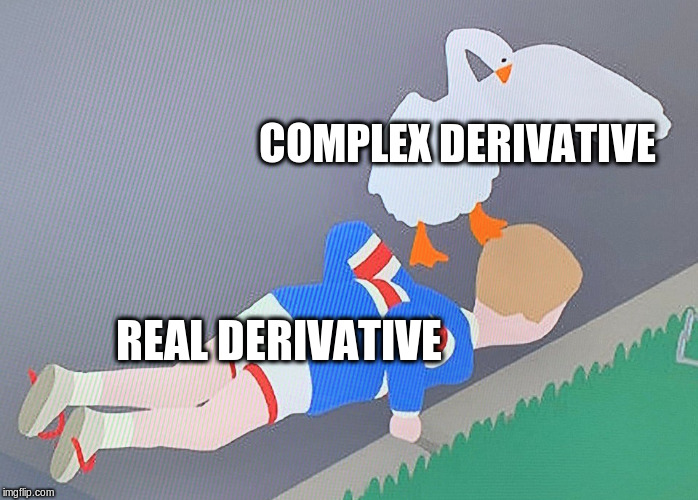
\includegraphics[width=\textwidth,height=0.8\textheight,keepaspectratio]{GooseDerivative.jpg}
\end{frame}


\begin{frame}{Line integrals: Another example}
  Consider the following two paths between 0 and $1+i$:
\begin{itemize}
\item $\alpha$ goes  along the circle of radius 1 centered at $i$
\item $\beta$ goes along the parabola $y=x^2$.
\end{itemize}

Compute:
\begin{enumerate}
\item $\int_\alpha \text{Re}(z) dz$
\item  $\int_\beta \text{Re}(z)dz$
\item $\int_\alpha zdz$
\item $\int_\beta zdz$
\end{enumerate}

What do you notice?
\end{frame}

\begin{frame}{Derivatives review}
\begin{definition} Let $f$ be defined on some open subset $U\subset \C$.  $f$ is \emph{differentiable} at $z_0\in U$ if
$$f^\prime(z_0):=\lim_{z\to z_0}\frac{f(z)-f(z_0)}{z-z_0}$$ 
exists.
\end{definition}
\begin{block}{Looks like normal derivative, but...}
\begin{itemize}
    \item Numerator and denominator will be complex numbers
    \item Have to get the same limit no matter how we approach $z_0$
\end{itemize}
\end{block}
\begin{definition} A function $f$ is holomorphic (the notes use analytic, which I'll rant about later) at $z_0$ if it is differentiable at every point in some neighborhood around $z_0$.
  \end{definition}

\end{frame}

\begin{frame}
  
\begin{center}

\Huge

\usebeamercolor[fg]{frametitle}
Clicker Session \\
Turning Point app or \\
ttpoll.eu 

\end{center}

\end{frame}

\begin{frame}{Cauchy-Riemann Equations}

\begin{theorem}[Cauchy-Riemann Equations]
Suppose $f(z)=u(x,y)+iv(x,y)$ is differentiable at $z_0$.  Then at 
$$\frac{\partial u}{\partial x}=\frac{\partial v}{\partial y}\quad\quad\frac{\partial u}{\partial y}=-\frac{\partial v}{\partial x}\quad \text{ at } z_0$$
\end{theorem}

\begin{proof}
Compute $f^\prime(z_0)$ in two different ways:
\begin{itemize}
    \item Keeping $x$ constant
    \item Keeping $y$ constant
\end{itemize}
\end{proof}

\end{frame}


\begin{frame}{More on Cauchy-Riemann}
\begin{block}{Complex formulation:}
Sometimes convenient to write both Cauchy-Riemann equations as one complex equation:
$$\frac{\partial f}{\partial x} = -i \frac{\partial f}{\partial y}$$
\end{block}


\begin{block}{Extension (non-examinable): Analytic functions are conformal}
In MAS211 you looked at the derivative of a map $f:\R^n\to\R^m$ as a linear map $Df:\R^n\to\R^m$, and hence as a matrix.  If $f:\C\to\C$ is differentiable at $z_0$, this linear map corresponds to multiplication by a complex number $z=a+bi$, and in matrix form this is:\newline

$$Df(z_0)=\begin{bmatrix} a & -b \\ b & a \end{bmatrix}=r\begin{bmatrix} \cos(\theta) & -\sin(\theta) \\ \sin(\theta) & \cos(\theta)\end{bmatrix}$$

Hence the derivative is a rotation + a scaling, and \emph{preserves angles}
\end{block}


\end{frame}

\begin{frame}{Motivation for an "application": PDEs}
The Laplacian operator, written $\nabla^2$ or $\Delta$, acts on functions $g:\R^2\to\R$ by
$$\nabla^2g=\nabla\cdot\nabla g=\frac{\partial^2 g}{\partial x^2}+\frac{\partial^2 g}{\partial y^2}$$
and occurs in many PDEs important in applied math.  

\begin{block}{Examples}
Let $f(x,y,t)$ be a function of two space variables and one time variable.
\begin{itemize}
    \item The heat equation $\frac{\partial f}{\partial t}=\nabla^2f$
    \item The wave equation $\frac{\partial^2 f}{\partial t^2}=\nabla^2f$
\end{itemize}
\end{block}
A steady state solution to either of these equations would be $\nabla^2f=0$.  
\end{frame}

\begin{frame}{Harmonic Functions}
\begin{definition}
A function $u:\R^2\to\R$ is \emph{harmonic} if $\nabla^2f=0$
\end{definition}

\begin{lemma}Let $f(z)=u(x,y)+iv(x,y)$ be analytic on a domain $D$.  Then $u$ and $v$ are harmonic on $D$
\end{lemma}
\begin{proof} Cauchy-Riemann equations + mixed partials are equal.
\end{proof}
This gives us lots of harmonic functions.  
\begin{block}{Does this give us \emph{all} harmonic functions?}
Given a harmonic function $u(x,y)$ on a domain, is it the real part of an analytic function $f(z)$?
\end{block}
\begin{block}{Complete answer next time!}
\end{block}

\end{frame}





\end{document}
